\documentclass{standalone}
\usepackage{tikz}
\usepackage{ctex,siunitx}
\setCJKmainfont{Noto Serif CJK SC}
\usepackage{tkz-euclide}
\usepackage{amsmath}
\usetikzlibrary{patterns, calc,3d}
\usetikzlibrary {decorations.pathmorphing,decorations.pathreplacing,decorations.shapes}
\begin{document}
\small
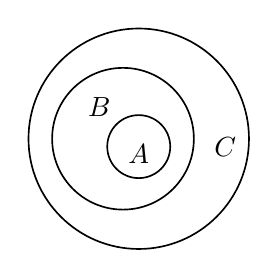
\begin{tikzpicture}[>=latex,scale=1.0]
  \draw[semithick](0,0)circle(0.4);
  \draw[semithick](-0.2,0.1)circle(0.9);
  \draw[semithick](0,0.1)circle(1.4);
  \node at (0,-0.1){$A$};
  \node at (-0.5,0.5){$B$};
  \node at (1.1,0){$C$};
\end{tikzpicture}
\end{document}